Before explaining RTSDP, we will first describe the SDP algorithm from~\cite{zamani12} and then explain how the XADD representation allows it to be efficiently performed.

\subsection{SDP Algorithm}

The symbolic dynamic programming (SDP) algorithm is a generalisation of the classical {\it value iteration} dynamic programming algorithm~\cite{bellman57} for constructing optimal policies for MDPs.
It proceeds by constructing a series of $h$ stages-to-go optimal value functions $V_h(\vec{b},\vec{x})$.
The pseudocode of SDP is shown in Algorithm \ref{alg:sdp}.
Beginning with $V_0(\vec{b},\vec{x}) = 0$ (line 2), it obtains the \emph{quality} $Q_{a(\vec{y})}(\vec{b},\vec{x})$ for each action $a(\vec{y}) \in \mathcal{A}$ (lines 5-8) in state $(\vec{b},\vec{x})$ by regressing the expected reward for $h-1$ future stages $V_{h-1}(\vec{b},\vec{x})$ along with the immediate reward $R(\vec{b},\vec{x},a(\vec{y}))$ as the following:
\begin{align}
Q_{a(\vec{y})}(\vec{b},\vec{x}) = & R(\vec{b},\vec{x},a(\vec{y})) + \sum_{\vec{b}'} \int_{\vec{x}'} \Bigg[ 
\prod_i \mathcal{P}(b_i' | a(\vec{y}),\vec{b},\vec{x}) \cdot  \nonumber \\  & \prod_j \mathcal{P}(x_j' | \vec{b'}, a(\vec{y}),\vec{b},\vec{x})\cdot V_{h-1}(\vec{b}',\vec{x}') \Bigg]. \label{eq:sdpregr} 
\end{align}

Given $Q_{a(\vec{y})}(\vec{b},\vec{x})$ for each $a(\vec{y}) \in A$, we can define the $h$ stages-to-go value function as the quality of the best action in each state $(\vec{b},\vec{x})$ as follows (line 7):
\begin{align}
V_{h}(\vec{b},\vec{x}) & = \max_{a(\vec{y}) \in A} \left\{ Q_{a(\vec{y})}(\vec{b},\vec{x}) \right\}. \label{eq:sdpmax}
\end{align}

The optimal value function $V_h(\vec{b},\vec{x})$ and optimal policy $\pi^*_h$ for each stage $h$ are calculated after $h$ steps. Note that the policy is obtained from the maximisation in Equation~\ref{eq:sdpmax}, $\pi^*_h(\vec{b},\vec{x}) = \argmax_{a(\vec{y})} Q_{a(\vec{y})}(\vec{b},\vec{x})$ (line 8). 
The regression step (Procedure 1.1) computes Equation \ref{eq:sdpregr} using the XADD data structure.

\vspace{-2mm}
%%%%%%%%%%%%%%%%%%%%%%%%%%%%%%%%%%%%%%%%%%%%%%%
\begin{algorithm}[ht!]
\small
\DontPrintSemicolon
\caption{\texttt{SDP}(HMDP M, $H$) $\rightarrow$ $(V^h,\pi^*_h)$ ~\cite{zamani12}\label{alg:sdp}}
\SetKwFunction{regress}{Regress}
\SetKwFunction{myproc}{\bf Procedure}{}{}
\SetKwFunction{remapWithPrimes}{Prime}
	$V_0:=0, h:=0$\;
	\While{$h < H$}{
		$h:=h+1$\;
		\ForEach {$a \in A$}{
			$Q_{a(\vec{y})} \gets\,$\regress{$V_{h-1},{a(\vec{y})}$}\;
		}
		$V_{h} \! \gets \! \max_{a(\vec{y})} \, Q_{a(\vec{y})}$ $\,$ \emph{// Maximize all $Q_{a(\vec{y})}$}\;
		$\pi^*_h \gets \argmax_{a(\vec{y})} \, Q_{a(\vec{y})} $\;
	}
	\Return{$(V_h, \pi^*_h)$} \;
\vspace{3mm}

\setcounter{AlgoLine}{0}
\myproc~{\bf 1.1}:~\regress{$V_{h-1}$, $a(\vec{y})$ }{

$Q=$ \remapWithPrimes{$V_{h-1}$} $\,$ \emph{// Rename all symbolic variables} 
- \hspace{25mm} \emph{// $b_i \to b_i'$ and all $ x_i \to x_i'$} \;
\ForEach { $b_i'$ in $Q$}  
    {
	\emph{// Discrete marginal summation, also denoted $\sum_{b'}$}\\
	$Q \gets \left[ Q \otimes P(b_i'|\vec{b},\vec{x},a(\vec{y})) \right]|_{b_i' = 1}$
	\mbox{$\;\;\;\;\;\;\;$}$\oplus \left[ Q \otimes P(b_i'|\vec{b},\vec{x},a(\vec{y})) \right]|_{b_i' = 0}$\;
}
	\ForEach { $x_j'$ in $Q$}  
{
	\emph{//Continuous marginal integration}\\
	$Q \gets subst_{x'_j = T_{a(\vec{y})}(\vec{b},\vec{x},\vec{b'})} Q $\;
}
	\Return{$Q \oplus R(\vec{b},\vec{x},a(\vec{y}))$}\;
}
\end{algorithm}
%%%%%%%%%%%%%%%%%%%%%%%%%%%%%%%%%%%%%%%%%%%%%%%
\vspace{-5mm}

\subsection{XADD representation}

The XADD data structure~\cite{sanner11} is used to efficiently represent and manipulate piecewise polynomial functions.
An XADD is a directed acyclic graph with two kinds of nodes, internal and terminal. Internal nodes are decision nodes that contain two edges, namely \emph{true} and \emph{false} branches, and a decision that can be either a boolean variable or a polynomial inequality on the continuous variables.
Terminal nodes contain a polynomial expression on the continuous variables.
XADDs represent piecewise functions by using decision nodes to separate regions and terminal nodes for the local functions (i.e. a expression valid inside a region).

For example, Figure~\ref{fig:exampleDD}(left) shows the plot of a piecewise function and Figure~\ref{fig:exampleDD}(right) its XADD representation.
Every path in an XADD defines a partial assignment of boolean variables and a continuous region that satisfies all inequalities in its internal nodes.
%If there are many regions with the same local function, then the paths will merge into a single terminal node, as in the dashed lines of Figure~\ref{fig:exampleDD} (right). 

The SDP algorithm uses four kinds of XADD operations: (i) Algebraic operations (sum $\oplus$, product $\otimes$) are naturally defined within each region, so the resulting partition is a cross-product of the original partitions and within each region the operation is straightforward. (See Figure \ref{fig:XADDadd}), (ii) Substitution operations (replacing or instantiating variables) affect both internal and terminal expressions and any decision that is no longer symbolic is replaced by the corresponding branch.(See Figure \ref{fig:XADDsubs}),
(iii) Comparison operations (maximisation) cannot be performed directly between terminal expressions so a new decision node comparing terminal expressions is created.(See Figure \ref{fig:XADDmax}),
(iv) Parameter maximization operations modify expressions substituting the maximal values and modify the structure adding comparisons between different branches (See Figure \ref{fig:XADDparamax}).
These XADD operations have been defined previously and we refer to~\cite{sanner11,zamani12} for details.
%%%%%%%%%%%%%%%%%%%%%%%%%%%%%%%%%%%%%%%%%%%%%%%
\begin{figure}[th]
\center
\vspace{-2mm}
\subfloat[Addition~($\oplus$).]{
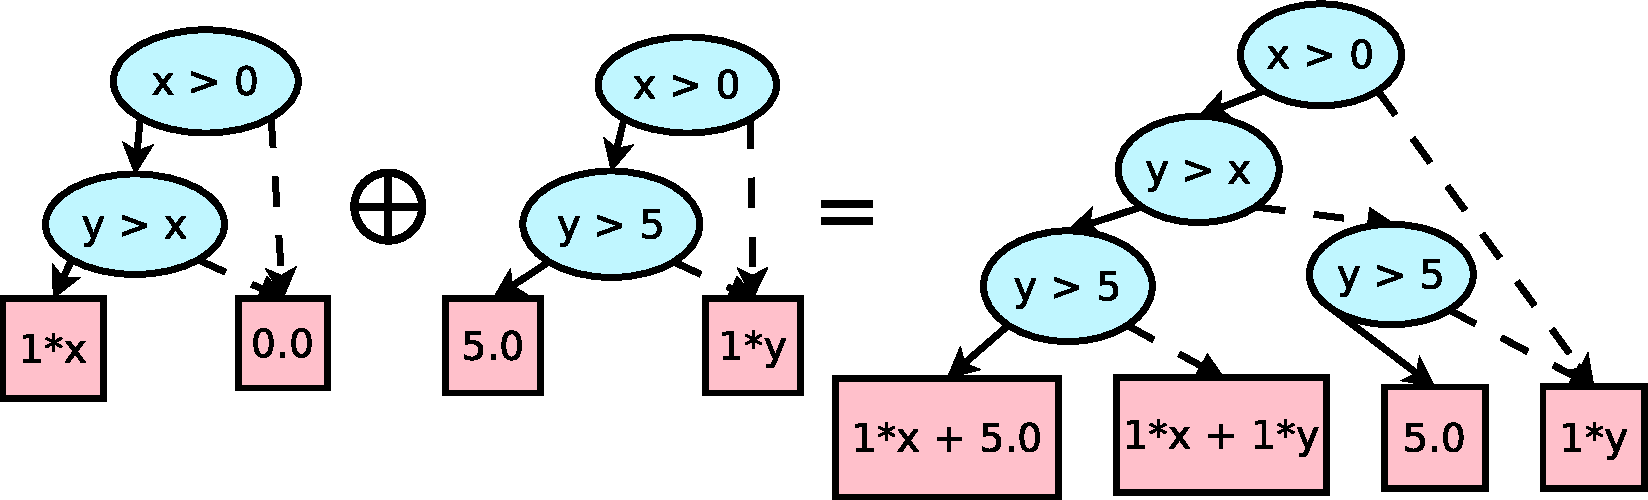
\includegraphics[width=0.45\textwidth]{figures/xaddOps/XADDsum.pdf} 
\label{fig:XADDadd}
}

\hspace{10mm}
\subfloat[Substitution~($subst$).]{
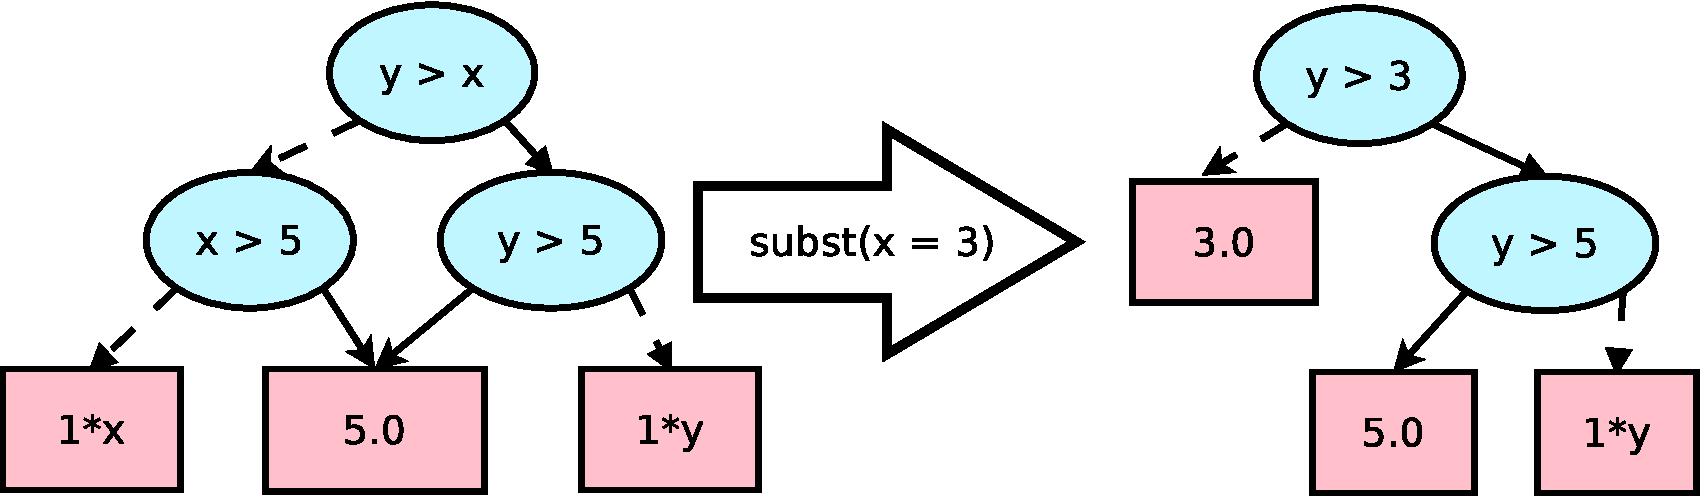
\includegraphics[width=0.45\textwidth]{figures/xaddOps/XADDsubs.pdf} 
\label{fig:XADDsubs}
}

\vspace{-4mm}
\subfloat[Maximisation~($\max$)]{
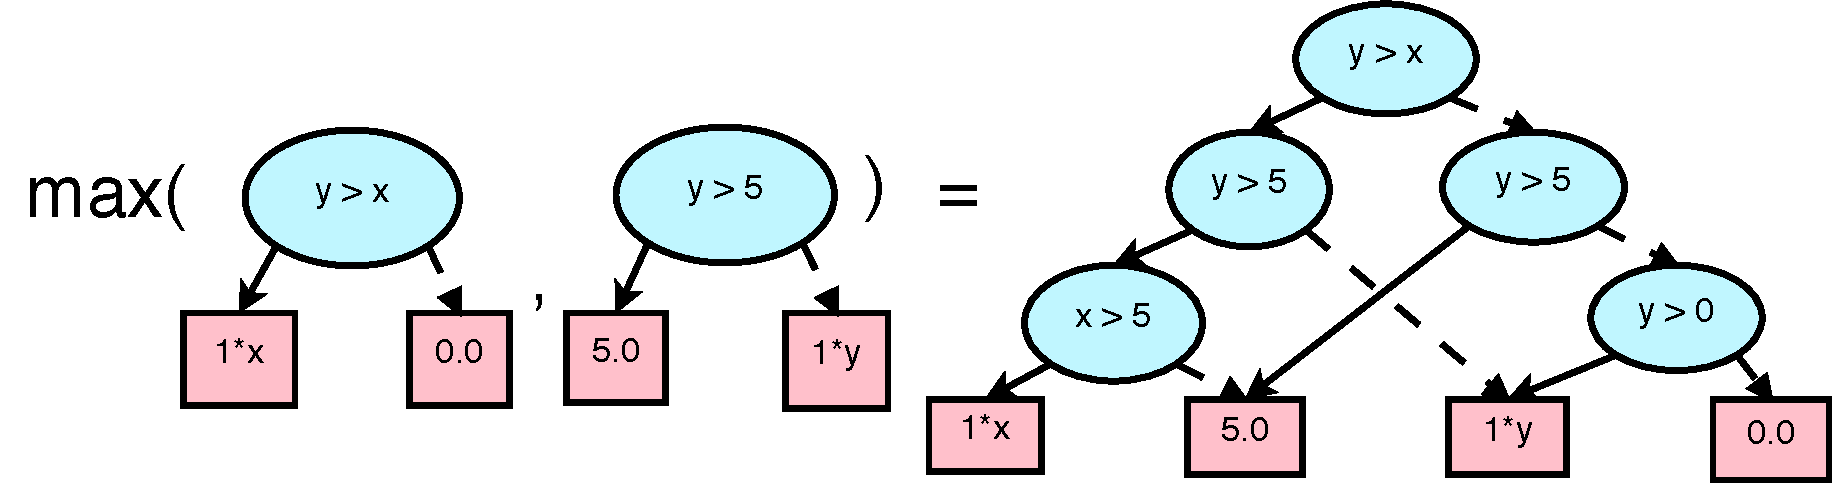
\includegraphics[width=0.45\textwidth]{figures/xaddOps/XADDmax.pdf} 
\label{fig:XADDmax}
}

\subfloat[Parameter Maximisation~($\pmax$).]{
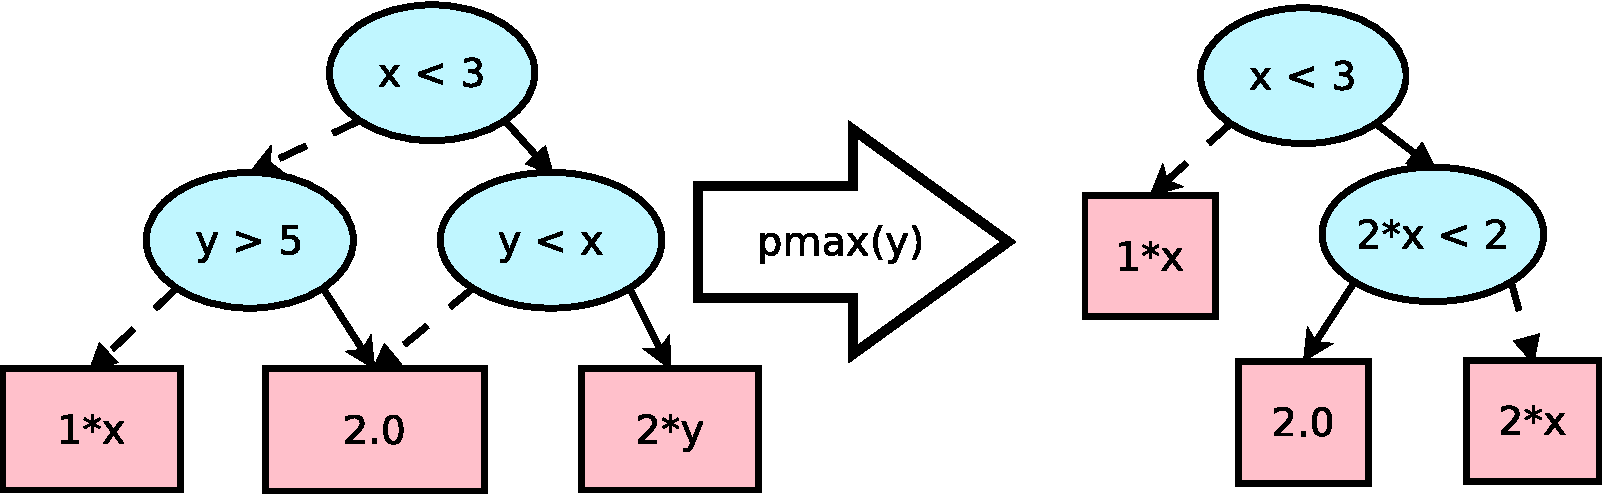
\includegraphics[width=0.4\textwidth]{figures/xaddOps/XADDpmax.pdf} 
\label{fig:XADDparamax}
}
\caption{XADD Operations.}
\vspace{-2mm}
\end{figure}
%%%%%%%%%%%%%%%%%%%%%%%%%%%%%%%%%%%%%%%%%%%%%%%

Thus, the SDP Bellman update (Equations \ref{eq:sdpregr} \& \ref{eq:sdpmax}) is performed synchronously as a sequence of XADD operations \footnote{$F^{DD(vars)}$ is a notation to indicate that $F$ is an XADD symbolic function of $vars$.}, in two steps:
\begin{itemize}
\item {Regression of all states:
\begin{align}
Q_a^{DD(\vec{b},\vec{x},\vec{y})} & =  R_a^{DD(\vec{b},\vec{x},\vec{y})} \oplus \nonumber \\
	& \hspace{-1.4cm}  \sum_{\vec{b}'}  P_a^{DD(\vec{b},\vec{x},\vec{y},\vec{b'})} \otimes \left[ subst_{(x' = T_a^{DD(\vec{b},\vec{x},\vec{y},\vec{b'})})} V_{h-1}'^{DD(b',x')} \right]. 
\label{eq:SDPregrDD}
\end{align}
}
\item{
Maximization for all states w.r.t. parametrised actions:
\begin{equation}
V_h^{DD(\vec{b},\vec{x})} = \max_{a} \left( \pmax_{\vec{y}}~ Q_a^{DD(\vec{b},\vec{x},\vec{y})} \right).
\label{eq:SDPmaxDD}
\end{equation}
}
\end{itemize}

As these operations are performed the complexity of the value function increases and so does the number of regions and nodes in the XADD. A goal of this work is to propose an efficient solution that avoids exploring unreachable or unnecessary regions.


